\documentclass[10pt,a4paper,twosided]{article}

\usepackage[margin=2cm]{geometry}
\usepackage{graphicx}
\usepackage[latin1]{inputenc}

\usepackage[titletoc]{appendix}
\usepackage{makeidx}
\usepackage{amsmath}
\usepackage{amssymb}

\usepackage{epic}
\usepackage{eepic}
\usepackage{float}

\usepackage{varioref}

\usepackage{listings,fancyvrb}
\usepackage{color}

\definecolor{dkgreen}{rgb}{0,0.6,0}
\definecolor{gray}{rgb}{0.5,0.5,0.5}
\definecolor{mauve}{rgb}{0.58,0,0.82}
\lstset{ %
  language=C++,                % the language of the code
  basicstyle=\footnotesize,           % the size of the fonts that are used for the code
  % numbers=left,                   % where to put the line-numbers
  numberstyle=\tiny\color{gray},  % the style that is used for the line-numbers
  % stepnumber=2,                   % the step between two line-numbers. If it's 1, each line 
                                  % will be numbered
  % numbersep=5pt,                  % how far the line-numbers are from the code
  backgroundcolor=\color{white},      % choose the background color. You must add \usepackage{color}
  showspaces=false,               % show spaces adding particular underscores
  showstringspaces=false,         % underline spaces within strings
  showtabs=false,                 % show tabs within strings adding particular underscores
  frame=single,                   % adds a frame around the code
  rulecolor=\color{black},        % if not set, the frame-color may be changed on line-breaks within not-black text (e.g. commens (green here))
  tabsize=2,                      % sets default tabsize to 2 spaces
  captionpos=b,                   % sets the caption-position to bottom
  breaklines=true,                % sets automatic line breaking
  breakatwhitespace=false,        % sets if automatic breaks should only happen at whitespace
  title=\lstname,                   % show the filename of files included with \lstinputlisting;
                                  % also try caption instead of title
  keywordstyle=\color{blue},          % keyword style
  commentstyle=\color{dkgreen},       % comment style
  stringstyle=\color{mauve}%,         % string literal style
  %escapeinside={\%*}{*)},            % if you want to add a comment within your code
  %morekeywords={*,...}               % if you want to add more keywords to the set
}

\renewcommand{\theenumi}{\roman{enumi}.}
\renewcommand{\labelenumi}{\theenumi}

% Which style to cite references
\usepackage{hyperref}
\def\bibname{References}
\usepackage[round]{natbib}
\bibliographystyle{plainnat}

\renewcommand{\cite}{\citep*}

\newcommand{\figuretext}[1]{\caption{\textit{#1}}}
\newcommand{\vct}[1]{\mathbf{#1}}

\title{Report project assignment PDC Summer school 2014}
\author{Andreas Karlsson and Niten Olofsson}


\begin{document}
\lstset{language=C++}

\maketitle

\thispagestyle{empty}

\tableofcontents


\abstract{}

\section{Introduction}

The software in question, microsimulation (ref to github), implements
a probabilistic model, on a person to person level, of the occurence
of prostate cancer in men from the age 35 and above. It also includes
means of modelling different health care policies (such as screening
of population at certain ages), the performance of the different tests
utilised, the probability that a person A with symptoms B seeks care
themselves, and so forth.

By generating a population, and performing microsimulation (ref),
i.e., follow each person (unit) over their life span, and then sort
the outcome in different predefined categories, the effect of
different policies are evaluated. This fulfills the criteria of the
MapReduce programming model \cite{MapReduce:2004}, where the
simulation is the map step, and the sorting into different categories
is the reduction step.

The software has been developed ``organically'' over the years, the
first version being implemented in C, then later in C++. It is called
from R, using the Rcpp (ref) package. If we can reduce the execution
time, and/or increase the sample size, different policies can be
evaluated, and better accuracy obtained.

We choose to first adapt the code to use OpenMP to see if any
improvements could be achieved, and if time permitted, OpenMP and
MPI. The first in order to decrease the execution time, and the second
to allow for much larger sample sizes. In the end, it turned out that
we only had time to adapt the code to OpenMP.


% % Description of the package and its architecture.
% Purpose 
% Package to perform so called microsimulation. Sample population is
% generated, using a probalistic model of prostate cancer, follows
% persons (micro unit). Implementing different so called policies
% regarding screening, treatment, and try to evaluate their effect in
% terms of survival rates, cost for health care and so forth.


% % Technical
% Invoked from R. Fulfills the map-reduce computational
% model/paradigm. (Describe how it fulfills the map-reduce paradigm).
% Reduce step is ensemble averages (c.f., micro vs. macro states in
% statistical physics; Sample population generation -> apply operation
% rules (map step), collect statistics according to the defined criteria
% (reduce step)).

% % Aim
% Shorten execution time drastically to be able to try out a large
% amount of different policies. Want to be able to run larger
% models. First aim, OpenMp, second aim means MPI or equivalent, i.e..


%%% Local Variables:
%%% mode: latex
%%% TeX-master: "report"
%%% End:


% Rekapitulering av vad vi gjorde

\section{Overview of the changes to the code}

The computation can be modelled using the MapReduce programming model. After
analysing the code base, the conclusion was to first try to
parallelise using openmp, then extend to MPI.

First, to the map step of the code, we added
%\lstset{language=C}
\begin{lstlisting}
#pragma omp parallel shared(nthreads,chunk) private(i,tid,sim,diffTime,cumTime)
...
#pragma omp for schedule(static,1).
\end{lstlisting}
However, the reduce step was not straight forward to parallelise. In
the serial version of the code, the result was accumulated in an
associative array (\texttt{map} in C++ terminology ) with scope
throughout the whole module file (\emph{source file}) , and every
simulation result was incrementally added to the end result
associative array. In this reduction step several function calls was
made updating the result object, where the functions accessed it in
the scope of the file and not by a passed reference. So in the first
naive version, we just added \lstset{language=C++}
\begin{lstlisting}
#pragma omp critical
  {
  // updating the result, i.e., ``reduction step''
    report.add(FullState(state, ext_grade,
               dx, psa>=3.0, cohort), msg->kind,
               previousEventTime, now());
  }
\end{lstlisting}
around the section accessing the resource.

After some performance analysis, we realised that the reduction step
as implemented became the bottle-neck of the whole program. Instead,
we let each thread/process build up its contribution to the resulting
associative array in a private variable, and then merge these partial
results into the shared result object.

The R software also have a feature of using multi-cores, and we used
that one as a benchmark to the minimum performance we should obtain.

Summarising the steps, we label them
\begin{enumerate}
\item naive OpenMP (parallelising the map step)
\item improved OpenMP (first a thread-wise partial reduction, then
  reducing these partial results)
\item R automatic multi-threading.
\end{enumerate}

% R parallelisation

%%% Local Variables:
%%% mode: latex
%%% TeX-master: "report"
%%% End:


\section{Performance}

From assignment:
Prioritize measurements and analysis/interpretation!

Demonstrate use of tools (profiling, ...) , and simple performance
model.

\subsection{Measurements}

\subsection{Profiling}

%%% Local Variables:
%%% mode: latex
%%% TeX-master: "report"
%%% End:


\section{Results}

\subsubsection{Motivational R-side measurements}

\begin{figure}[!htbp]
  \centering
  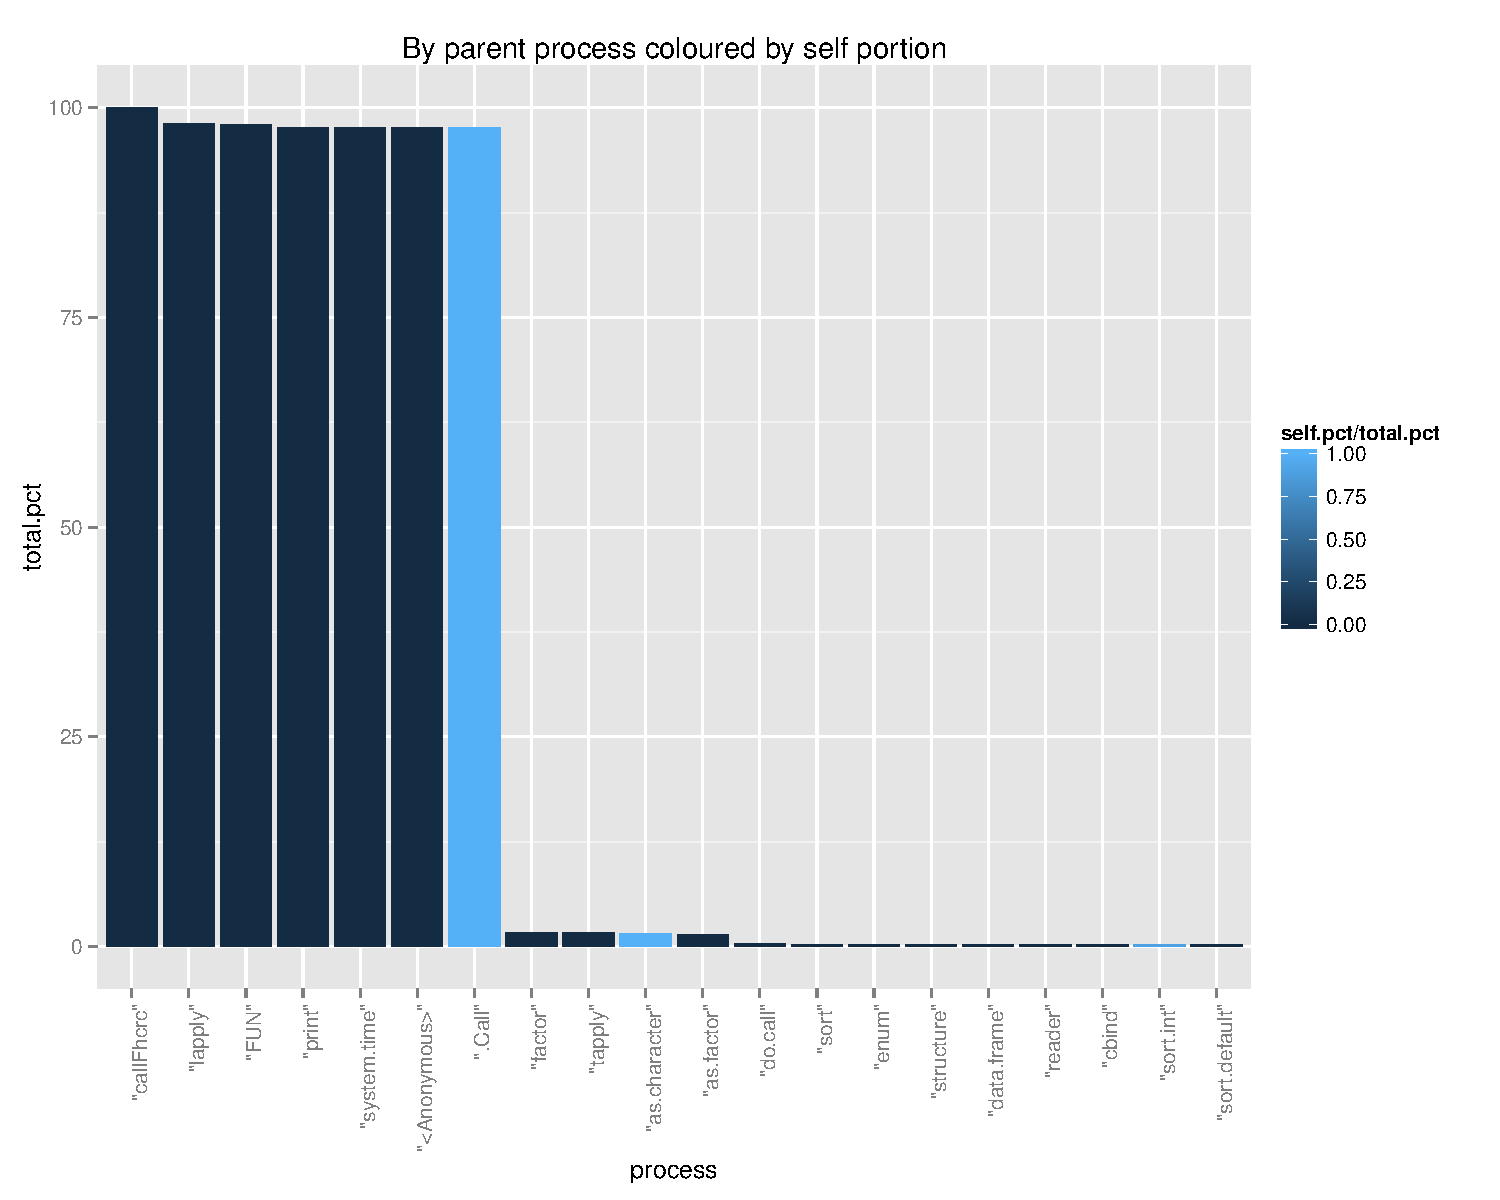
\includegraphics[width=0.7\textwidth]{images/parentColByPortion.pdf}
  \caption{Performance testing on the R side, where the ".Call" is
    the C++-code which can be run in parallel.}
  \label{fig:Rself}
\end{figure}

To motivate the need and choice to go parallel Figure \ref{fig:Rself})
shows the processes from the R-side where ".Call" is the part
which is implemented in C++ and which can be run in parallel.

\subsection{Baseline measurements C++}

\begin{figure}[!htbp]
  \centering
  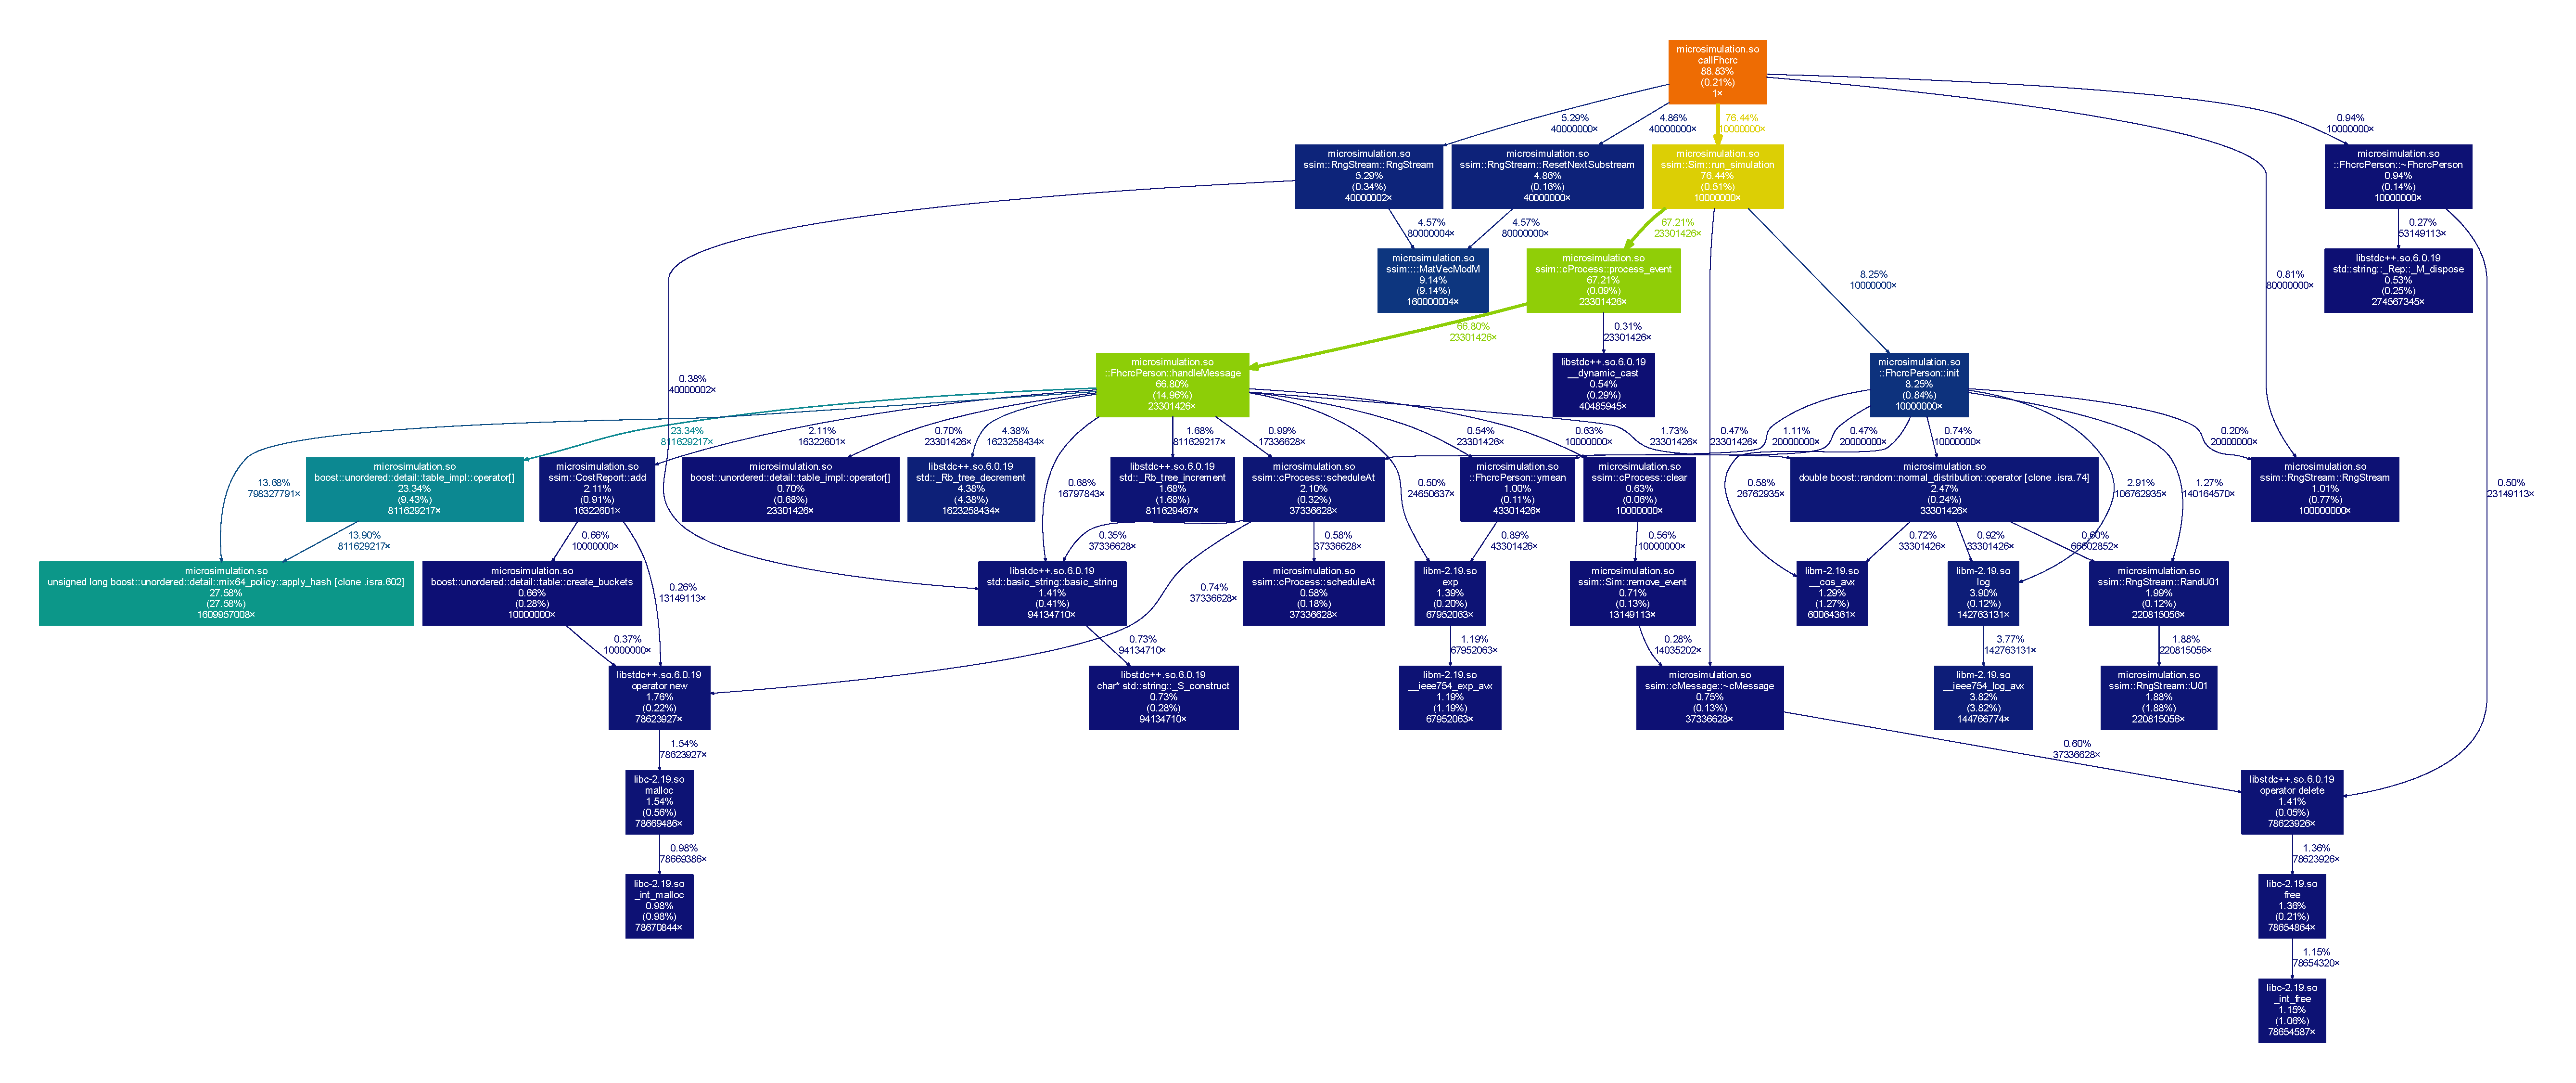
\includegraphics[height=0.50\textheight, angle=90]{images/profBaseLine.pdf}
  \caption{Valgrind measurements at baseline}
  \label{fig:simpleOpenMP}
\end{figure}


\subsection{Simple approach with OpenMP}

\begin{figure}[!htbp]
  \centering
  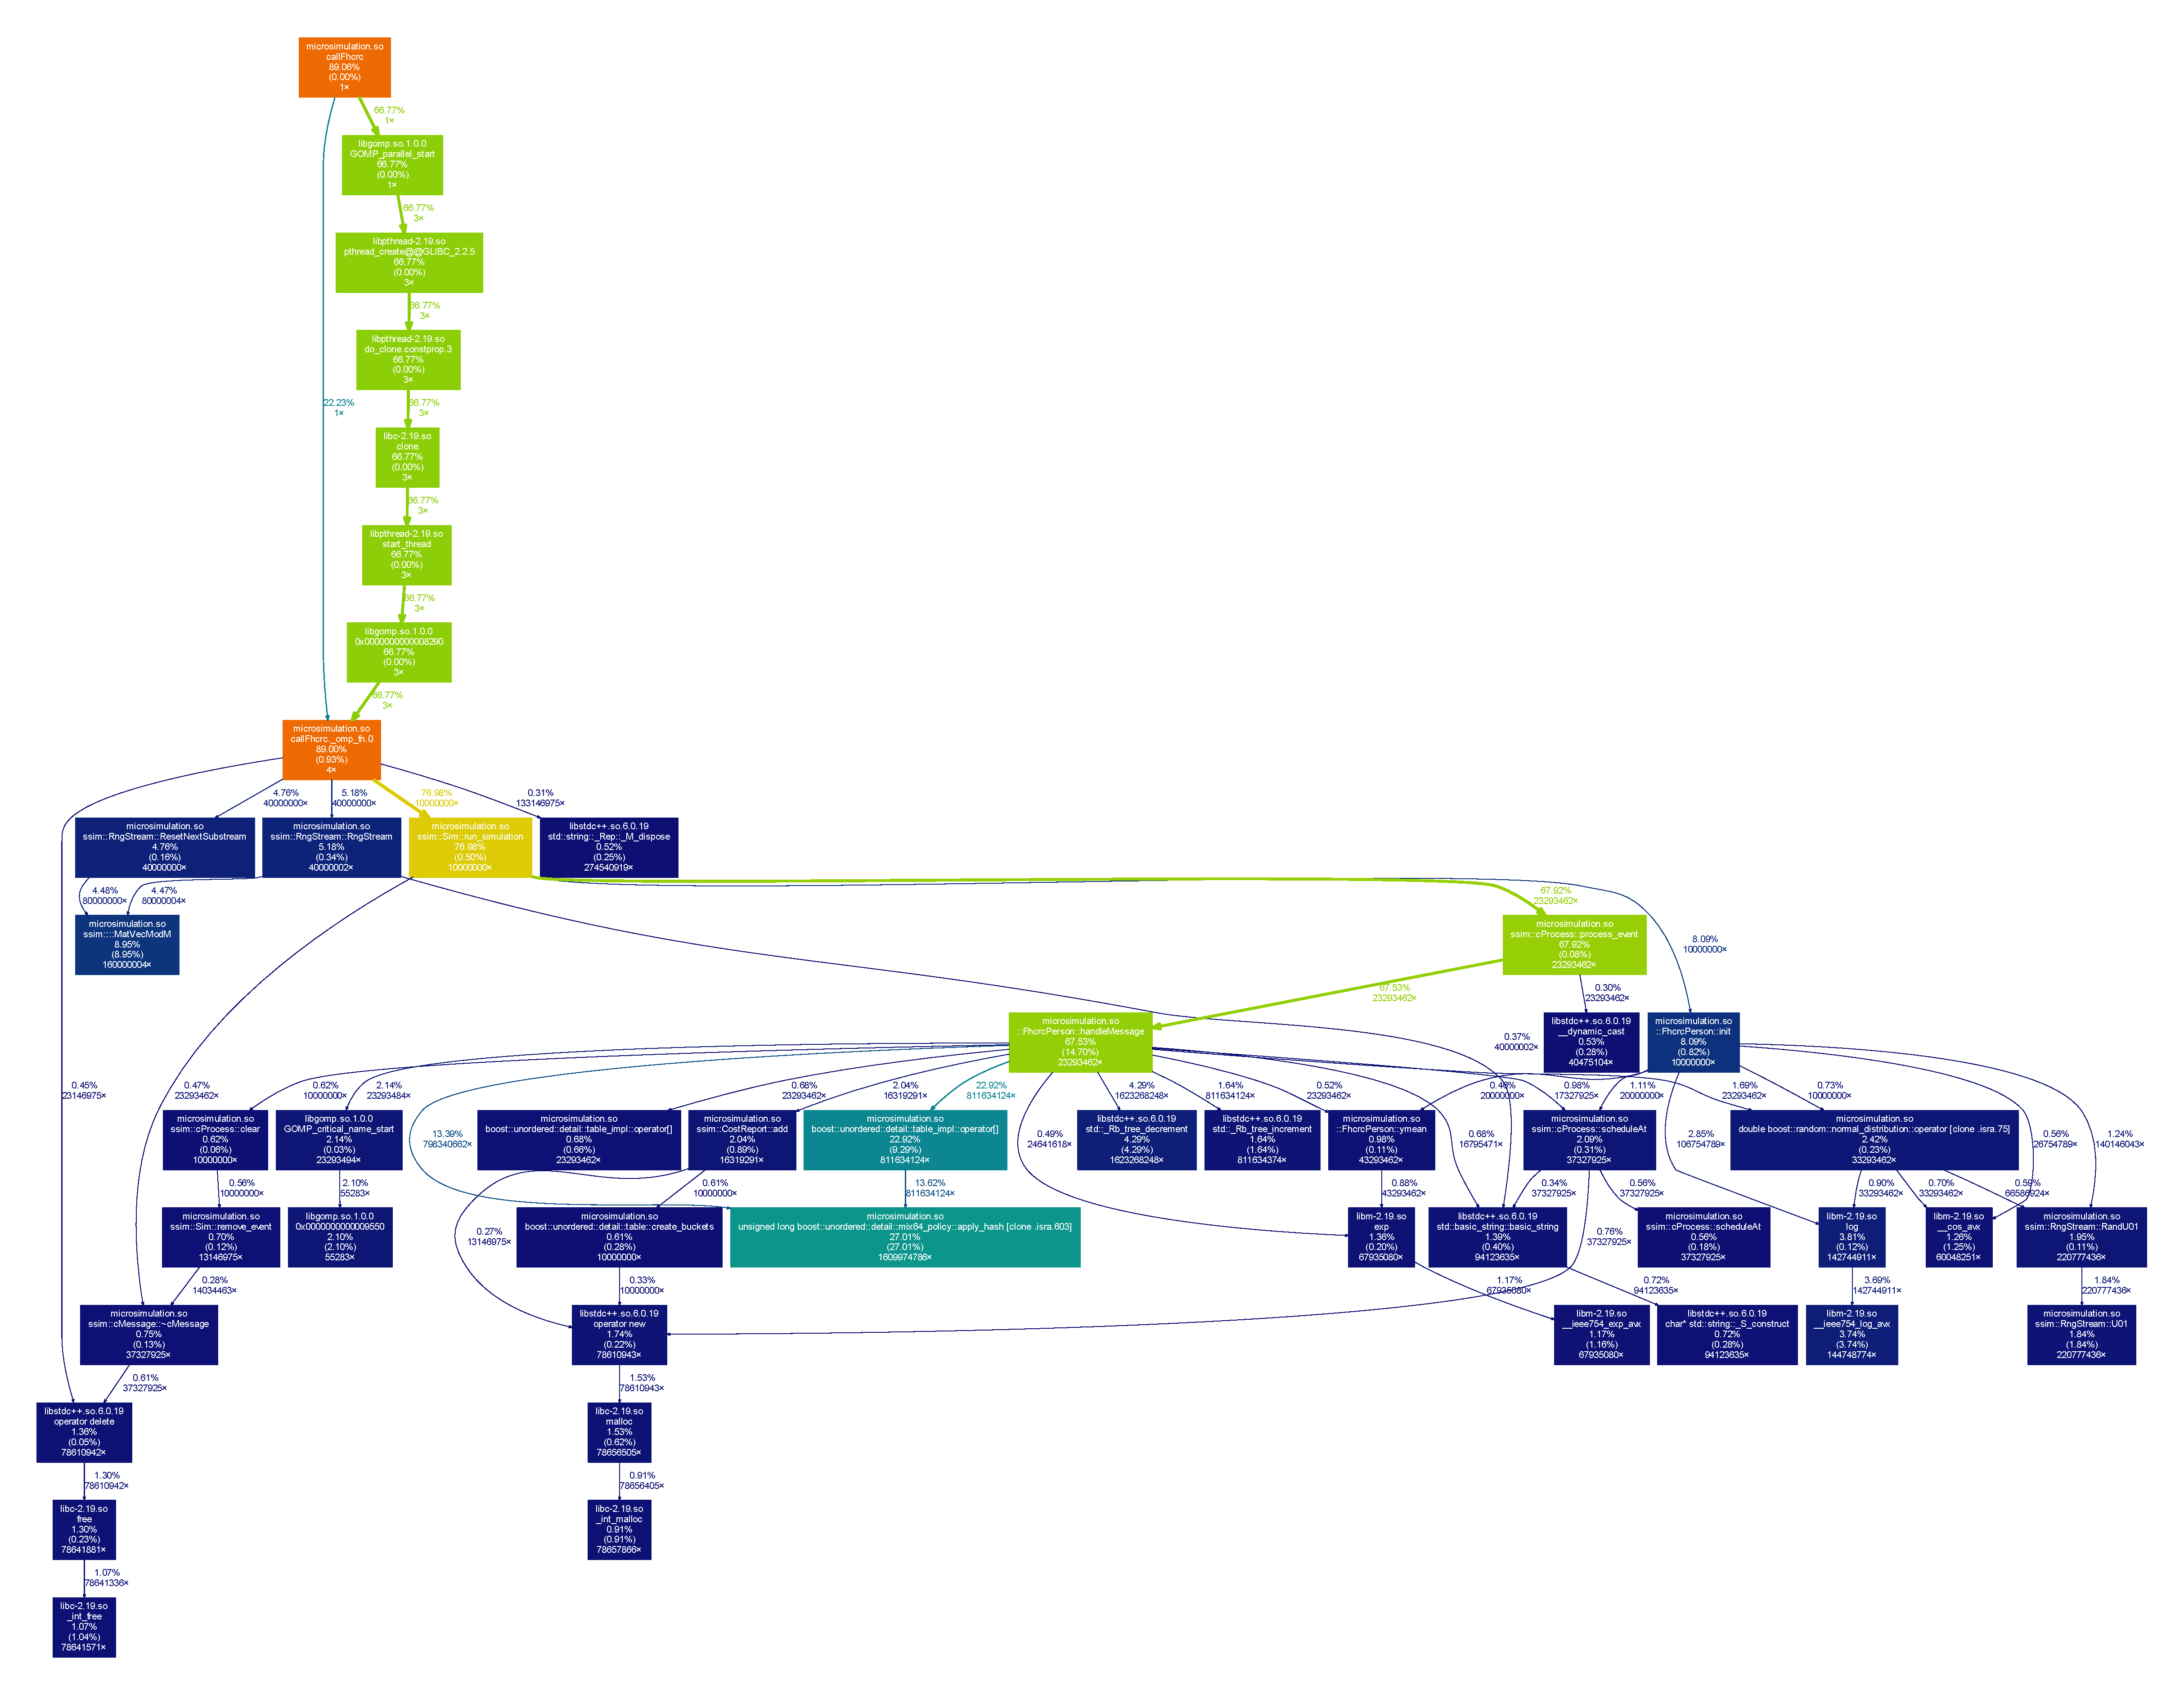
\includegraphics[height=0.85\textheight, angle=90]{images/profOpenMPSimple.pdf}
  \caption{Valgrind results of the simple openMP implementation}
  \label{fig:simpleOpenMP}
\end{figure}

Here the simulation loop is run in parallel whereas the data output
and some post-processing is run within a omp critical statement.

\subsection{Data output in parallel}


\subsection{Hybrid openMP and MPI}


%%% Local Variables:
%%% mode: latex
%%% TeX-master: "report"
%%% End:

\subsection{Three shared memory implementations}

We have compared three different implementation for shared memory parallelisation: 
\begin{enumerate}
\item ``R-side parallelism'', a high level R multi-threading which uses
  \texttt{mclapply} from the R \texttt{parallel} package.
\item ``naive openMP'' which encloses the map step with \texttt{\#pragma
    omp parallel} and \texttt{\#pragma omp for}, and protects the
  global report object (reduction step) with \texttt{\#pragma omp
    critical}
\item ``improved openMP'', where the reduction step was refactored by
  first performing a thread-wise reduction in a thread-private report
  object and then finally reduced in the end report.
\end{enumerate}
\begin{figure}[!htbp] \centering
  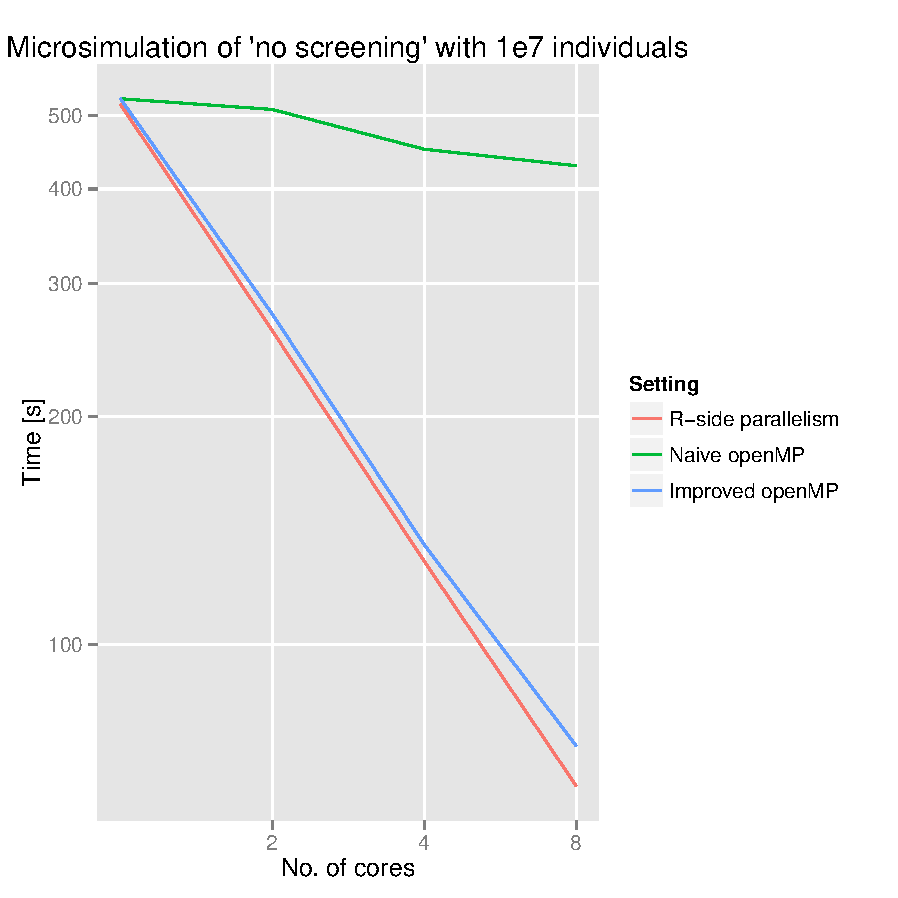
\includegraphics[height=0.5\textheight]{images/implementationProfiling.pdf}
  \caption{The execution times of the three different implementations
    described in the text. The difference between the ``naive openMP''
  and ``improved openMP'' is the local update to the report
  object.}
  \label{fig:implScaling}
\end{figure} 
Figure \ref{fig:implScaling} shows how the three
different implementations of parallelisation scales with additional
cores. The ``R-side parallelism'' and ``Improved openMP'' scales
well with comparable results. The ``Naive openMP'' implementation
with the ``EventReport'' mentioned in Figure \ref{fig:cppMot} within
\texttt{\#pragma omp critical} statements scales very poorly. 

Given the data, the automatic R-side parallelism should be
used. However, it does not scale beyond a single node, so if one wants
to run a significant larger population, then the combination \texttt{openMP
+ MPI} could be used.


%%% Local Variables: 
%%% mode: latex 
%%% TeX-master: "report" 
%%% End:

\subsection{Compilation flags}

\begin{figure}[!htbp] \centering
  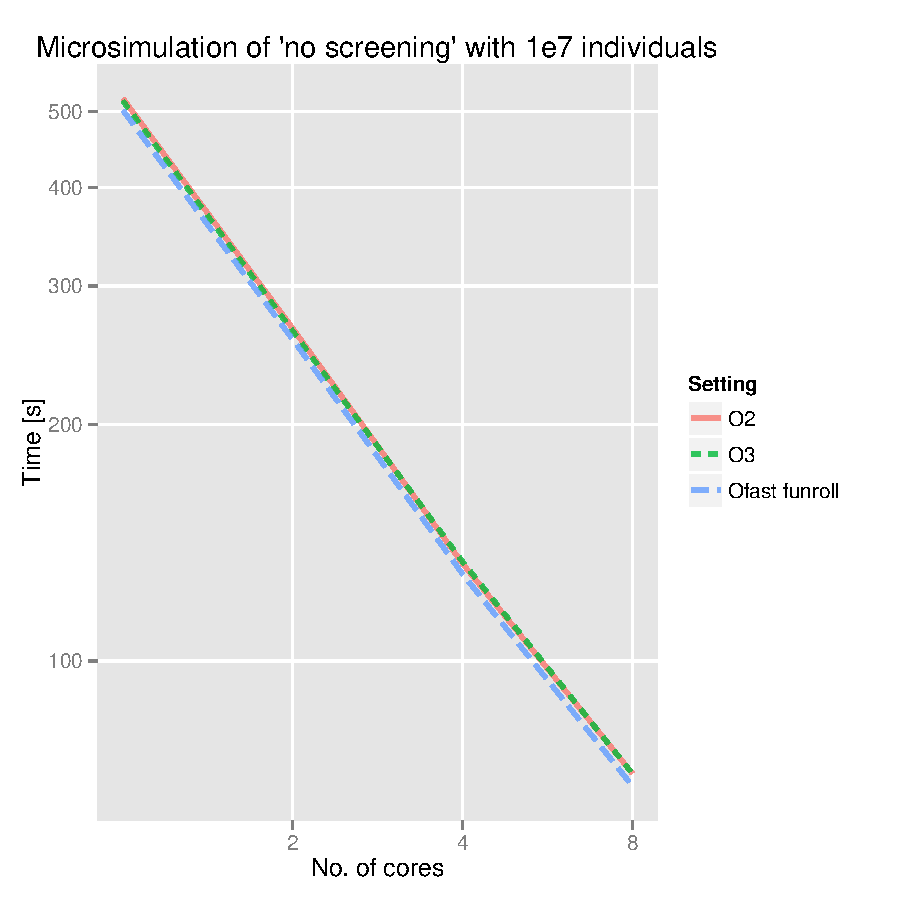
\includegraphics[height=0.5\textheight]{images/flagsProfiling.pdf}
  \caption{optimisation flags...}
  \label{fig:flagScaling}
\end{figure}


\subsection{Hybrid openMP and MPI}



%%% Local Variables: 
%%% mode: latex 
%%% TeX-master: "report" 
%%% End:


{\markboth{References}{References}
   \bibliography{references}
   }

\clearpage 
\begin{appendices}
%% Niten: fixar s� att appendix blir ett appendix
\section{Baseline profiling with Valgrind}
\label{sec:valgrind}
\begin{figure}[!htbp]
  \centering
  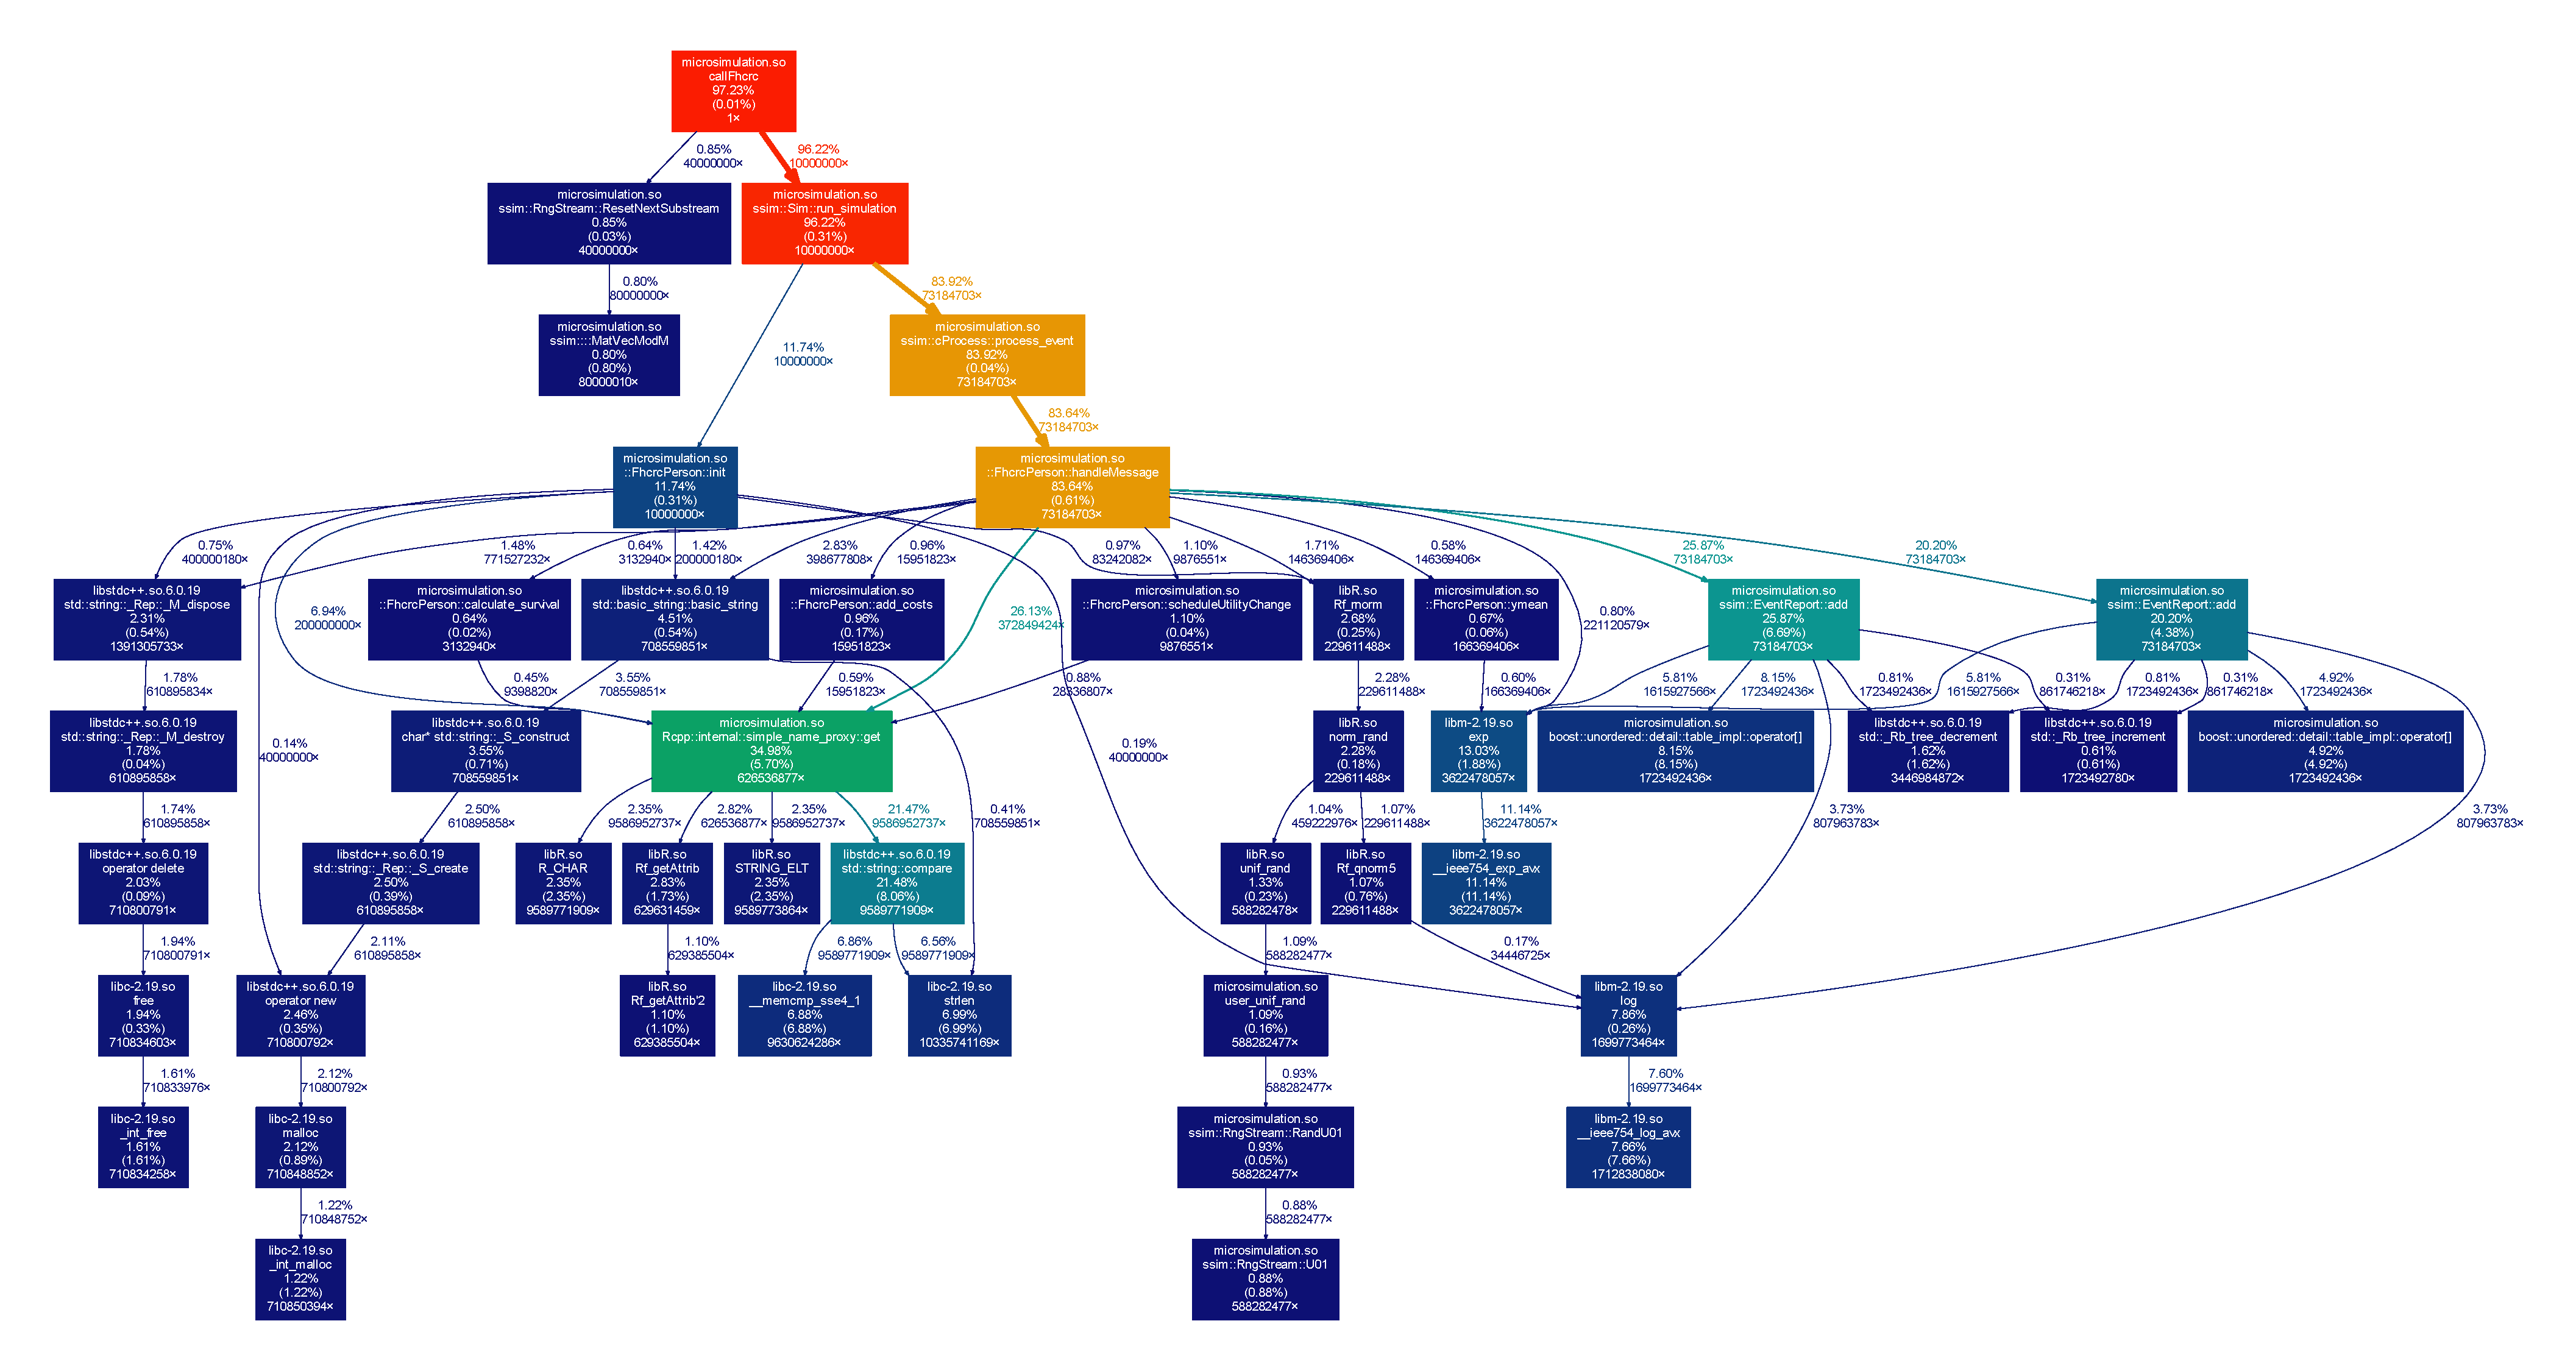
\includegraphics[height=0.45\textheight, angle=90]{images/mediumMotivationalValgrind.pdf}
  \caption{Valgrind measurements at baseline, more extensive then the
    image included in the report.}
  \label{fig:mediumValgrind}
\end{figure}

% \section{Baseline measurements C++}

% \begin{figure}[!htbp]
%   \centering
%   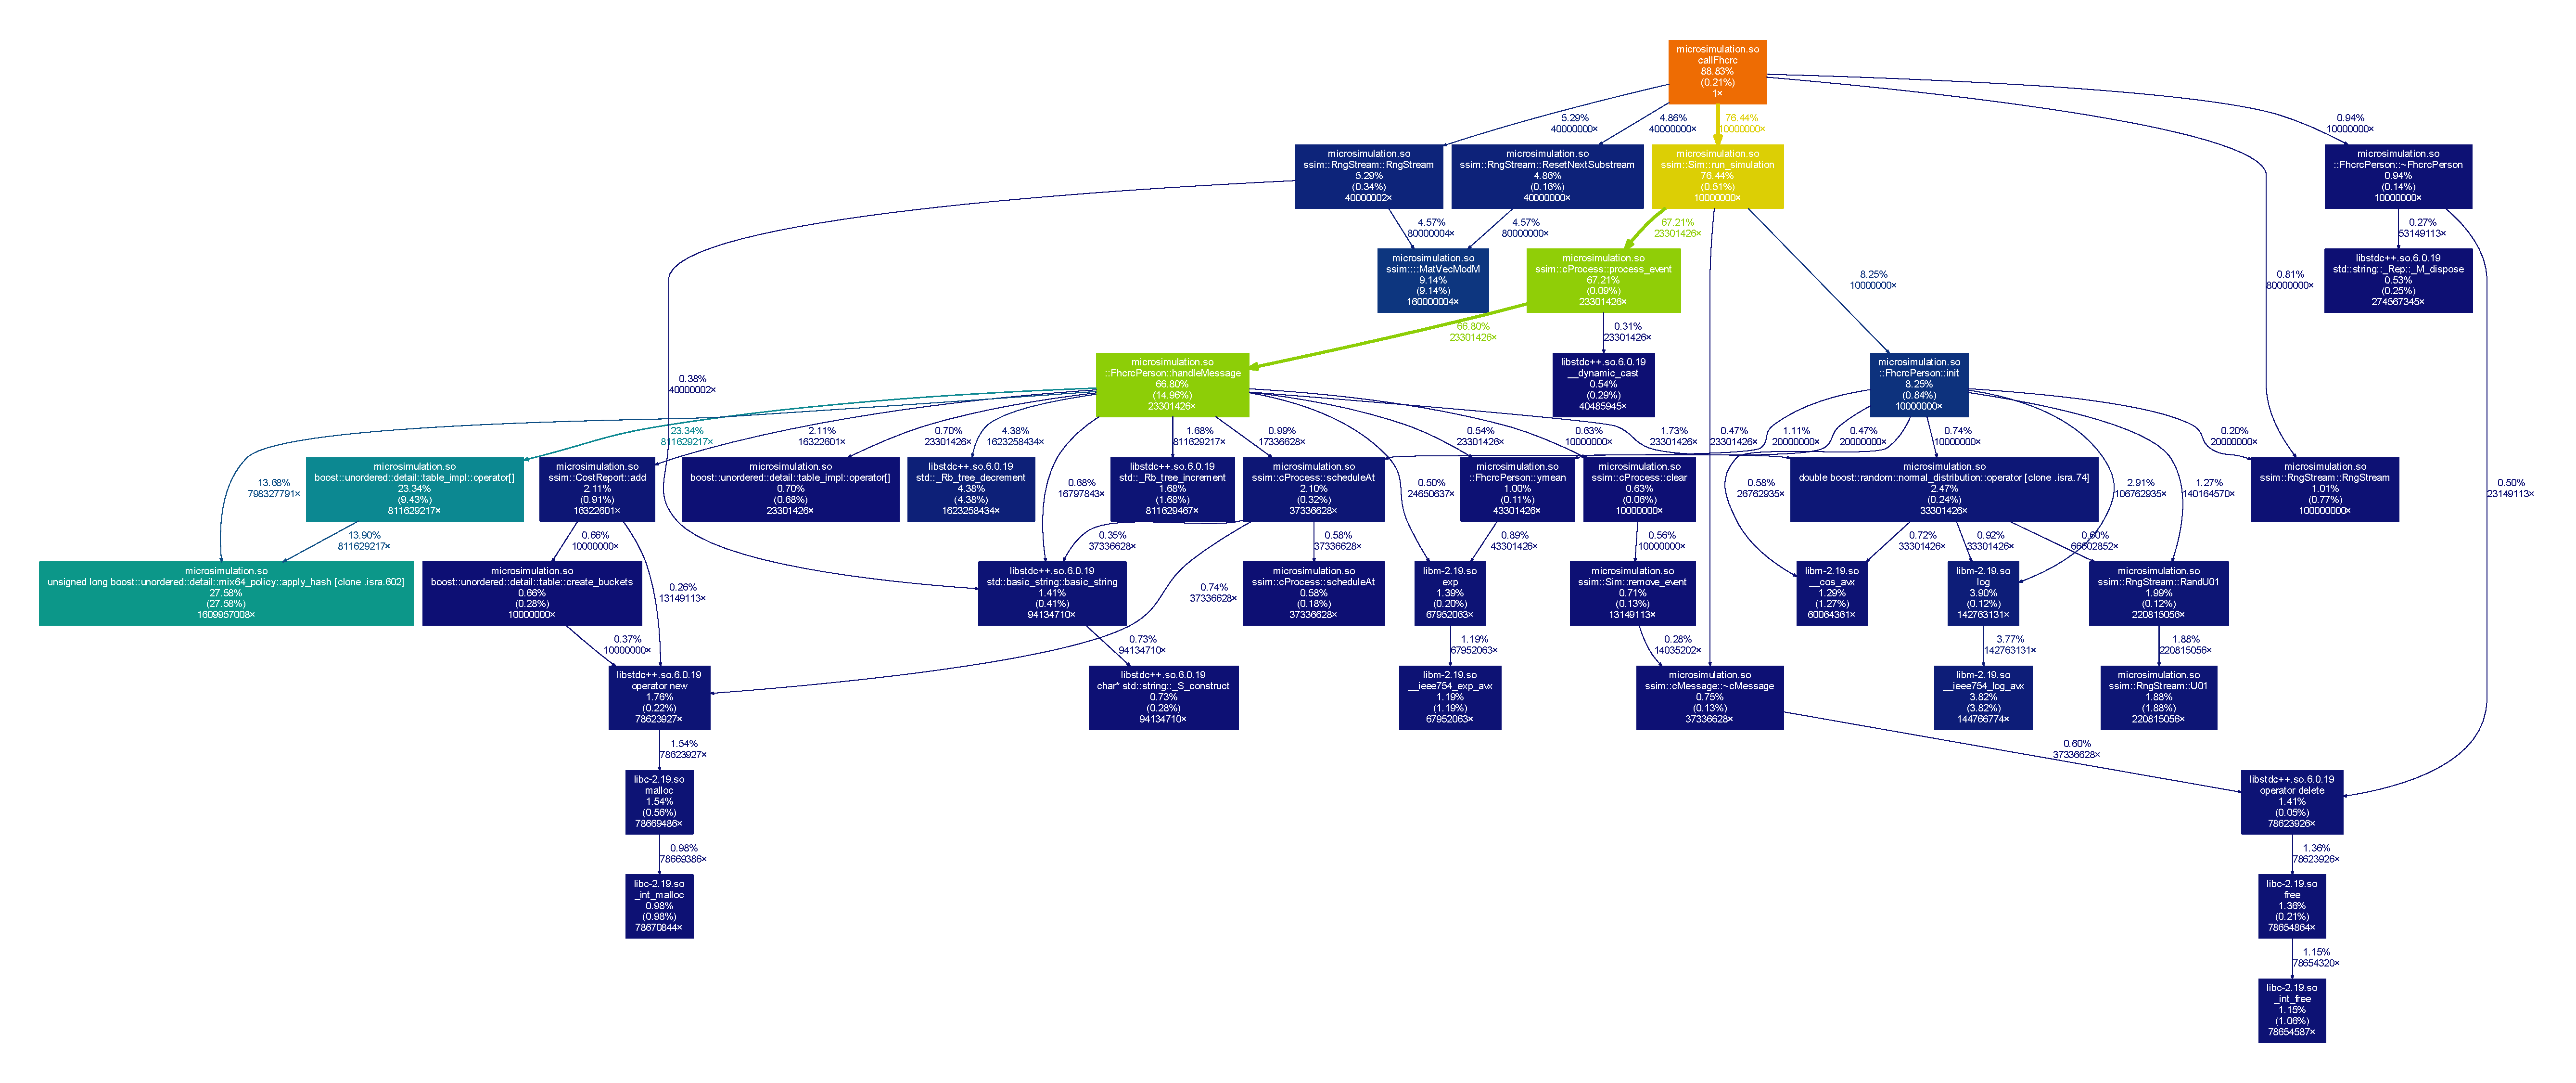
\includegraphics[height=0.50\textheight, angle=90]{images/profBaseLine.pdf}
%   \caption{Valgrind measurements at baseline}
%   \label{fig:baseline}
% \end{figure}


% \section{Simple approach with OpenMP}
% \begin{figure}[!htbp]
%   \centering
%   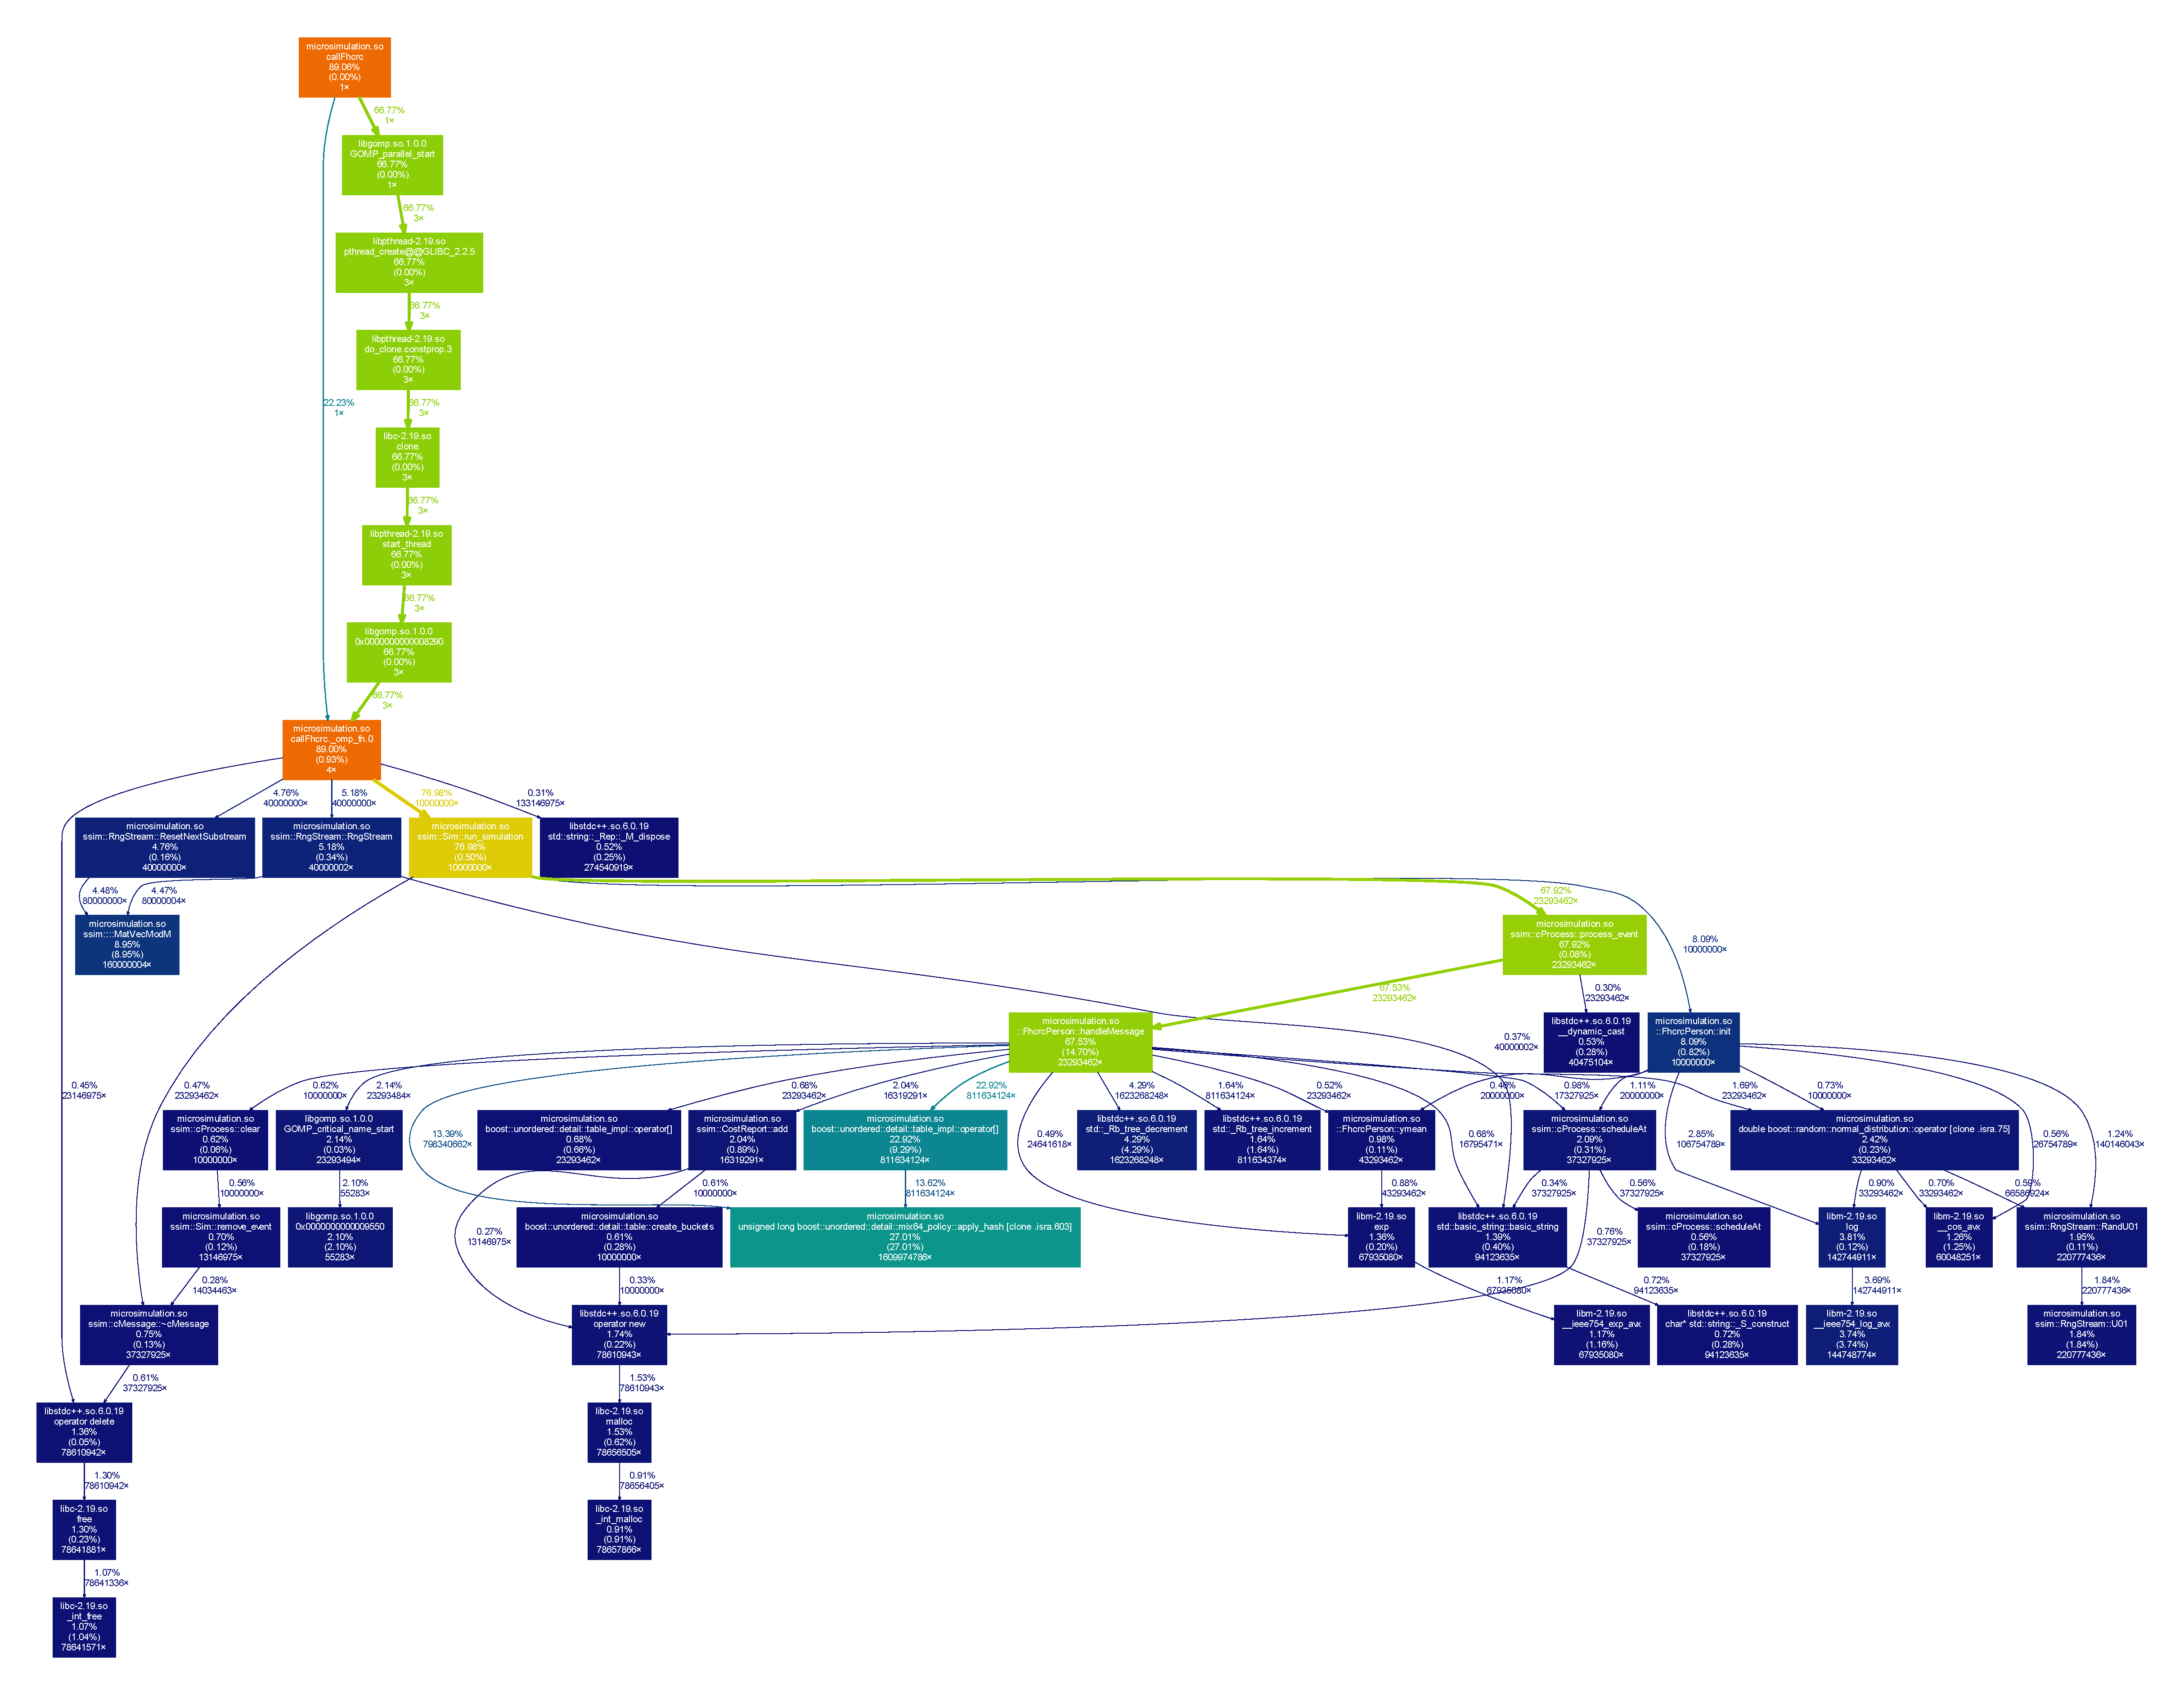
\includegraphics[height=0.85\textheight, angle=90]{images/profOpenMPSimple.pdf}
%   \caption{Valgrind results of the naive openMP implementation}
%   \label{fig:naiveOpenMP}
% \end{figure}

% Here the simulation loop is run in parallel whereas the data output
% and some post-processing is run within a omp critical statement.

%%% Local Variables:
%%% mode: latex
%%% TeX-master: "report"
%%% End:


\end{appendices}



\end{document}
